

\documentclass{article}
\usepackage{float}
\usepackage{amsmath,amssymb,amsthm,graphicx}
\usepackage{subcaption}
\usepackage{mleftright}

\setlength{\oddsidemargin}{0.25 in}
\setlength{\evensidemargin}{-0.25 in}
\setlength{\topmargin}{-0.6 in}
\setlength{\textwidth}{6.5 in}
\setlength{\textheight}{8.5 in}
\setlength{\headsep}{0.75 in}
\setlength{\parindent}{0 in}
\setlength{\parskip}{0.1 in}

\newtheorem{theorem}{Theorem}
\newtheorem{corollary}{Corollary}
\newtheorem{proposition}{Proposition}
\newtheorem*{remark}{Remark}
\theoremstyle{definition}
\newtheorem{example}{Example}
\newtheorem{definition}{Definition}

\newcommand{\lecture}[4]{
   \pagestyle{myheadings}
   \thispagestyle{plain}
   \newpage
%   \setcounter{lecnum}{#1}
   \setcounter{page}{1}
   \noindent
   \begin{center}
   \framebox{
      \vbox{\vspace{2mm}
    \hbox to 6.58in { {\bf CSC~565: Graph Theory
                        \hfill North Carolina State University} }
    \hbox to 6.58in { {\bf Fall 2019
                        \hfill Computer Science} }
       \vspace{4mm}
       \hbox to 6.28in { {\Large \hfill Lecture #1: #2  \hfill} }
       \vspace{2mm}
       \hbox to 6.28in { {\it Lecturer: {\it Don Sheehy {\tt <drsheehy@ncsu.edu>}} \hfill Scribe: #4} }
      \vspace{2mm}}
   }
   \end{center}
   \markboth{Lecture #1: #2}{Lecture #1: #2}
   \vspace*{4mm}
}


\begin{document}
    \lecture{20}{Oct 30, 2019}{}{Calvin Nguyen, Niharika Acharya, Shreeya Singh Dhakal}
    
    \section{Overview}
    In the previous lecture we discussed Maxwell-Cremona correspondence, projections of planar graphs to 3-dimensional space and correspondences between equilibrium stress and reciprocal diagrams, and liftings and reciprocal diagrams. In this lecture we continue from there and discuss Steinitz's theorem.
    

    \section{Steinitz's Theorem}
    Steinitz's theorem characterises simple, planar, 3-connected graph formed by the edges and vertices of a convex 3-dimensional polytope. 
    
    Statement: Every simple, planar, 3-connected graph can be realized as the edge skeleton of a convex 3-dimensional polytope. 
    
    
    
    \begin{figure}[H]
        \centering
        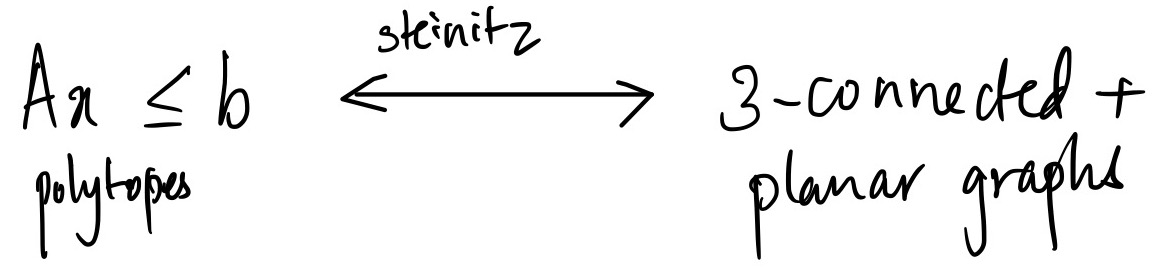
\includegraphics[width=.5\linewidth]{steinitz.JPG}
    \label{fig:steinitz}
    \end{figure}
    
    \textit{Note: In terms of algebra, a polytopal graph is represented by the set of solution to $Ax \leq b$}.
    
    Proof: We will prove Stienitz's theorem through Maxwell's correspondence that we studied in the previous lecture. 
     
     \textit{Revision: Maxwell-Cremona Correspondence: There is a natural correspondence between the equilibrium stress of straight-line drawing of a planar graph and its lifting.}
     
     \begin{figure}[H]
        \centering
        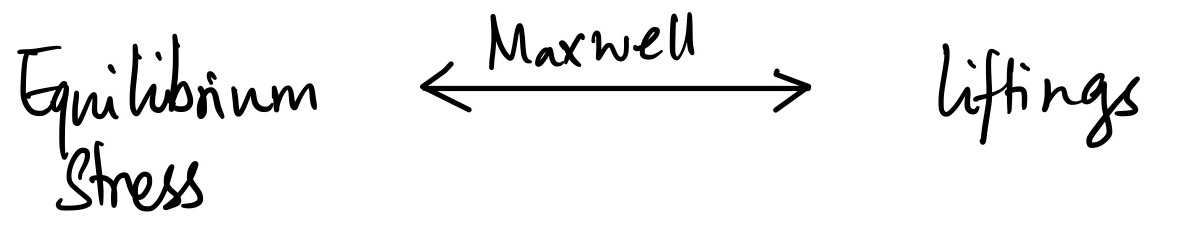
\includegraphics[width=.5\linewidth]{maxwell.JPG}

        \label{fig:maxwell}
    \end{figure}
     
     Consider a 3-connected, planar graph $G$. Say we draw $G$ such that all its edges are in equilibrium. Lifting up $G$ would give a Polytope. 
     
     \begin{figure}[H]
        \centering
        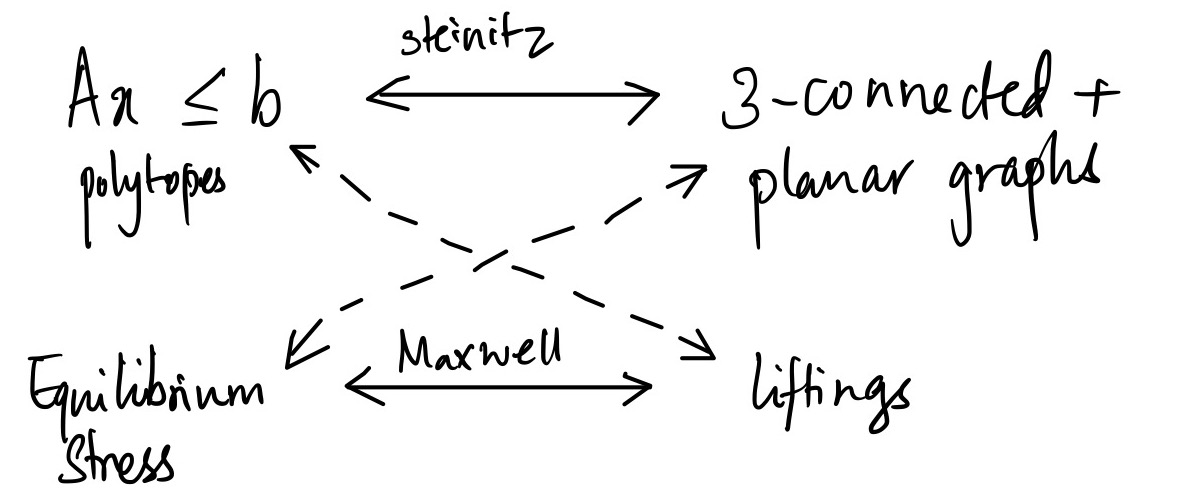
\includegraphics[width=.5\linewidth]{steinitz-proof.JPG}

        \label{fig:steinitz-proff}
    \end{figure}
     
     However, it is important to know a way to draw $G$, such that it is 3-connected, planar and with all forces in equilibrium. Tutte's spring embedding is a way to draw such graph.
     
    \section{Tutte's Spring Embedding:}
    Tutte's spring embedding of a 3-connected planar graphs is a linear embedding where faces are convex polygons.
    
    Consider a planar, 3-connected graph $G$. Select a face and fix its vertices to form a convex polygon. The edges of the face corresponds to the edges of the polygon. Each of the other vertex goes at the barycenter i.e the center of gravity of its neighbours. 
    
    Since, in the embeddings the edges are thought of as springs, we will look into Hooke's law, which can be used to find spring force of each edges to get a 3-connected, planar graph with net forces along the edges in equilibrium.
    
    
    \section{Hooke's Law}
    Statement: Hooke's Law states that the force F needed to extend or compress a spring by some distance x scales linearly with respect to that distance.
    Consider two vectors x and y.
    \newline The force of y on x is given by 
    \begin{figure}[h!]
            \centering
            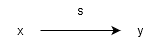
\includegraphics[scale=.7]{Hooke'sLaw.png}
    \end{figure}
    \newline F = s(y-x) 
    
    where s is the spring constant.
    
    We can find equilibrium relative to the spring constants. The assignment of spring constants to the edges is called a stress.
    
    \begin{figure}[h!]
            \centering
            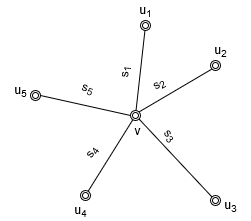
\includegraphics[scale=.7]{Hooke'sLaw2.png}
    \end{figure}
    \newline The total force on v is
    
    \newline F = $\sum_{i=1}^{5} s_i(u_i-v)$ 
    
    \newline If the system is in equilibrium then,
    
    \newline F = $\sum_{i=1}^{5} s_i(u_i-v)$ = 0
    
    The sum of the forces gives us the force polygon which is the dual of faces in the reciprocal diagram from Maxwell's correspondence.
    
    \newline In Tutte's algorithm,
    \newline We can chose any stresses we want, as long they are positive they will all bend the same way and it will correspond to a convex lifting. Let us pick the stresses to be 1. 
    
    \newline All spring constants = 1, except we wont consider the edges on the outer face
    
    \begin{figure}[H]
            \centering
            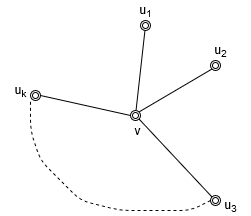
\includegraphics[scale=.7]{Hooke'sLaw3.png}
    \end{figure}
    
    Consider k such vectors from $u_1$ to $u_k$ such that s_1= s_2 = s_3...=s_k = 1 \\
    \newline F = $\sum_{i=1}^{k} s_i(u_i-v)$ \\
    \newline F = $\sum_{i=1}^{k} (u_i-v)$ \\
    \newline F = $\sum_{i=1}^{k} (u_i) - $\sum_{i=1}^{k} v  \\
    \newline F = $\sum_{i=1}^{k} (u_i)$ - deg(v)v  \\
    
    where deg(v) = k in this case. \\
    
    From the above equation we can say that this is a linear combination of points.\\
    Hence for the force to be equal to zero, we have linear equation to be satisfied.\\
    
    \section{Full Equilibrium Stress}
    Let P be position of each point. If each point $P_i$ is written as $x_i$, $y_i$ then,
    
    P = \begin{bmatrix} x_1\hspace{0.1cm} y_1\\\vdots\\ x_n\hspace{0.1cm}y_n\end{bmatrix}
    
    where P is a n x 2 matrix.\\
    
    The forces are 2D vectors. If the force vectors add up to zero, then the change is x coordinates add up to zero and the change in y coordinates add up to zero.\\
    
    Thus the linear combination of positions should add up to zero.
    
    -LP = 0 = Force = $R^{\mathrm{n x 2}}\\$ where,
    
    
    \newline L = some linear combinations of the positions\\
    F = n x 2 vector that denotes the net force on each vertex
    
    \section{Graph Laplacian}
    From the above equation, we get
    
    \[{L_{ij}}^{'}=\left\{\begin{array}{cl} deg(v_i),&i = j\\ -1,&(v_i,v_j)\in E\\ 0&\mbox{elsewhere}\end{array}\right.\] 
    
    
    The above matrix is called the \textbf{Graph Laplacian Matrix}
    
    Example: \\
    Consider a graph G,
    \begin{figure}[H]
            \centering
            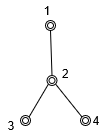
\includegraphics[scale=.7]{GraphLaplacianExample.png}
            \caption{G}
    \end{figure}
    
    Graph Laplacian of G,\\
    
    L =\begin{bmatrix} 1&-1&0&0 \\ -1&3&-1&-1\\ 0 &-1&2&-1 \\ 0&-1&-1&2 \end{bmatrix} \\
    
    The diagonal elements have i=j, hence are degrees of v \\
    For each edge in G, we have L[i,j] = -1 \\
    The above matrix is a symmetric matrix.\\
    
    The above Laplacian matrix can also be written as,
    
    L = D - A \\
    where,\\
    D = Diagonal matrix of the degrees of v \\
    A - Adjacency matrix \\
    
    Consider the problem in one dimension,
    LX = 0
    where L is linear combination of x coordinates that add up to zero.
    
    \textbf{Question}: Can the above graph G have a non trivial solution such that F=0?
    
    \textbf{Answer:} No, because of the one force at vertex 1. We can get F=0 only if the force at vertex 1 is 0. 
    
    \begin{remark} The Laplacian matrix is diagonally dominant i.e for each row the diagonal entry is greater than or equal to the sum of magnitudes of all other non diagonal entries in that row.
    \end{remark}
    
    The above Laplacian matrix for graph G, is not invertible. If you consider the sum of elements for every row in the above matrix L, they add up to 0.\\
    Hence det(L) = 0 and L is not invertible.
    
    As the sum of elements in each row in L is 0 we get the below equation,
    
    L \begin{bmatrix} 1\\1\\1\\1\end{bmatrix} = 0
    
    From the above solution,
    
    P = \begin{bmatrix} 1\\1\\1\\1\end{bmatrix}
    
    The above solution is a non-trivial solution but is a degenerate solution.\\
    Putting everything at one point we get the distances between each point as 0 and hence the net force is 0. \\
    \begin{remark}
    The above solution where you put everything at one point is the only non-trivial solution for the above Laplacian matrix L. There is no way to arrange the above spring system so that it is in equilibrium.
    \end{remark}
    
    \section{Finding an invertible sub-matrix in L}
    Let there be h vertices on the outer face or outer hull. \\
    Vertices on outer face = \{V1, V2, ..., ${V_h}$\} \\ 
    Other vertices = \{$V_{h+1}$,...$V_n$\} \\
    
    L = \begin{bmatrix} $L_1$ & B\\$B^T$ & $L_2$\end{bmatrix} \\
    
    where, 
    $L_1$ = h x h matrix corresponding to the first h rows and h columns \\
    
    We also know that any face can be the outer face. In algorithm, if we have fixed the positions of vertices on the outer face, we do not have choice for the positions of other vertices.
    
    LP = net force = 
\renewcommand\arraystretch{1.3}
\mleft[
\begin{array}{c|c}
  \L_1 & B \\
  \hline
  B^T & L_2
\end{array}
\mright]
\renewcommand\arraystretch{1.3}
\mleft[
\begin{array}{c}
  R \\
  \hline
  P
\end{array}
\mright]
 = \renewcommand\arraystretch{1.3}
\mleft[
\begin{array}{c}
  F \\
  \hline
  0
\end{array}
\mright]
  
    where, \\
    R = positions of the vertices of the outer face \\
    P = positions of all the inner vertices i.e all the vertices except for outer face\\
    F = net force on the outer face \\
    
    Expanding the above equation, we get, \\
    \newcommand{\dd}[1]{\mathrm{d}#1}
    \begin{equation}
    L_1R + BP = F \\    
    \end{equation}
    \begin{equation}
    B^TR + L_2P = 0 \\    
    \end{equation}
    
    We have chosen R as where we decide to put the outer face. \\
    In the second equation, we therefore know $B^T$ and we know R.
    
    \begin{equation}
    P = {-L_2}^{-1}(B^TR) \\    
    \end{equation}
    
    From the above equation, we need to calculate the inverse of $L_2$. We know that matrix L was not invertible as det(L) = 0. Let us now prove that matrix $L_2$ is invertible.
    
    \section{Matrix Tree Theorem}
    
    \begin{definition} Spanning tree is a tree which is a subgraph that touches all the vertices in G.
    \end{definition}
    
    Given a graph G and its Laplacian L,
    let $L'$ be the matrix with first row and first column removed from L, then\\
    det($L'$) = \# of distinct spanning trees in G
    
    \subsection{Tutte's argument on the invertibility of ${L_2}$}
    
    1) If you were to contract the outer face to a single vertex, then it is a connected graph.\\
    2) The Graph Laplacian is some Graph Laplacian for this new graph.\\
    3) If we remove this one vertex, the rest of the Laplacian would remain unchanged.\\
    4) $L_2$ is just the edges between the vertices that are not on the outer face.\\
    5) We defined faces in 3 connected, planar graphs as one whose removal leaves us with a connected graph.\\
    6) Hence removal of the vertices that make up the outer face leaves us with a connected graph.\\
    7) Each connected graph contains at least one spanning tree.\\
    8) Hence the graph that we get after removing the outer face contains at least one spanning tree.\\
    Hence the determinant value of ${L_2}$ is at least 1.\\
    9) Hence there is a non-singular matrix at ${L_2}$\\
    
    The above result proves that matrix ${L_2}$ is invertible. This gives us a drawing, but we wanted an embedding i.e a drawing where no edges cross and where faces as convex polygons.
    
    \section{Proving the drawing is planar and faces are convex polygons}
    \subsection{Monotone Paths}
    
    \begin{figure}[H]
            \centering
            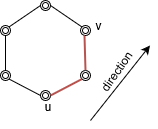
\includegraphics[scale=.7]{monotonepaths.png}
    \end{figure}
    
    
    Consider vertices u and v and a direction, we can always find a path from u to v in the direction. These paths are called as monotone paths. \\
    If we have a polytope, there exist monotone paths in every direction.\\
    There exist monotone paths to the outer face.\\
    
    We can also think about them in the following way,
    \begin{figure}[h!]
            \centering
            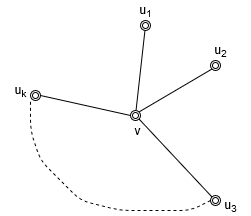
\includegraphics[scale=.7]{Hooke'sLaw3.png}
    \end{figure}
    
    In the above figure, if the net force is 0, then 
    
    $\sum_{i=1}^{k} (u_i-v)$ = 0 \\
    
    $\sum_{i=1}^{k} (u_i) - kv = 0 \\
    
    kv = $\sum_{i=1}^{k} (u_i)\\
    
    v = 1/k * $\sum_{i=1}^{k}(u_i)
    
    The point v is called as the mean or the centroid or the barycenter.\\
    If the net forces are zero then each of the vertices which are not on the outer face are exactly at the centroid of its neighbors.\\
    
    \begin{figure}[h!]
            \centering
            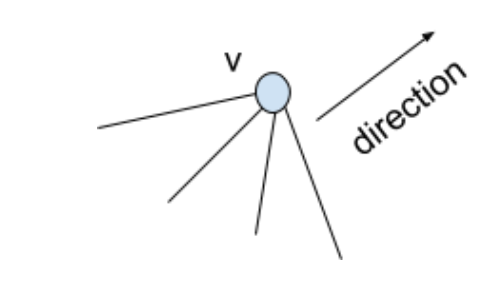
\includegraphics[scale=.7]{barcycenter.PNG}
            \caption{v is not at the centroid of the neighbors}
    \end{figure}
    
    If there is no monotone path from v in the above direction, it would mean that all of the neighbors of v are on the opposite side. And clearly v is not at the centroid of the neighbors.\\
    
    Hence all monotone paths go out till the outer face.
    We also know that the non separating induced cycles in 3 connected planar graphs are the faces.\\
    We can pin one of the faces as the outer face and get monotone paths to this outer face.\\
    
    \subsection{Non convex faces and Windings}
    
    These monotone paths will help us check that the drawing is really a convex representation in the following way. 
    
    Consider the following figures, \\
    Case 1: Non convex face with zig zag edges
        
    
    \begin{figure}[h!]
            \centering
            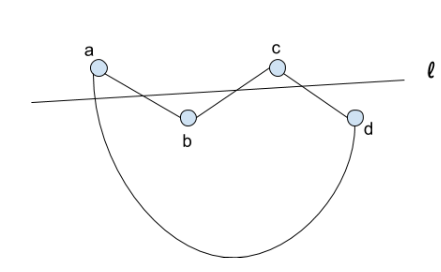
\includegraphics[scale=.7]{monotone_1.PNG}
            \caption{A non convex face}
    \end{figure}
    
    \begin{figure}[h!]
            \centering
            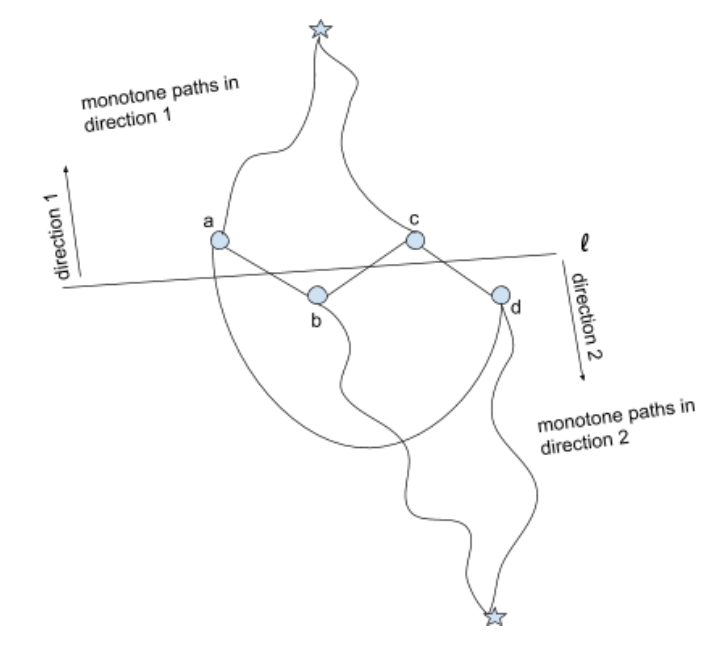
\includegraphics[scale=.7]{monotone_2.PNG}
            \caption{Monotone paths meeting at outer face}
    \end{figure}
    
    The face F formed by the vertices is non convex. Let line l separate the vertices such that vertex a,b are one side of the line and vertex c,d are on opposite side of the line. There are monotone paths from vertices a and c in direction 1. Suppose they reach the farthest vertex on the outer face and intersect at point denoted by a star. Similarly, monotone paths from b and d in the direction 2 intersect at some point denoted by star. The paths from a to c and from b to d are disjoint because they are monotone. If they were not monotone they would have to cross the line.\\
    The above graph formed by vertices a,b,c,d is K4 since monotone paths connect a to c and b to d.
    
    \begin{figure}[H]
            \centering
            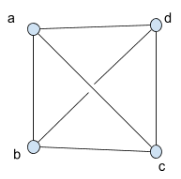
\includegraphics[scale=.7]{k4.PNG}
            \caption{K4: a non outer planar graph}
    \end{figure}
    
    Since K4 is not outer planar, the vertices a,b,c,d cannot be on the same face. This gives us contradiction since we assumed a,b,c,d was a face. Hence all the faces are convex. 
    
    \textbf{Case 2: Non convex faces with windings}
    
    
    \begin{figure}[H]
            \centering
            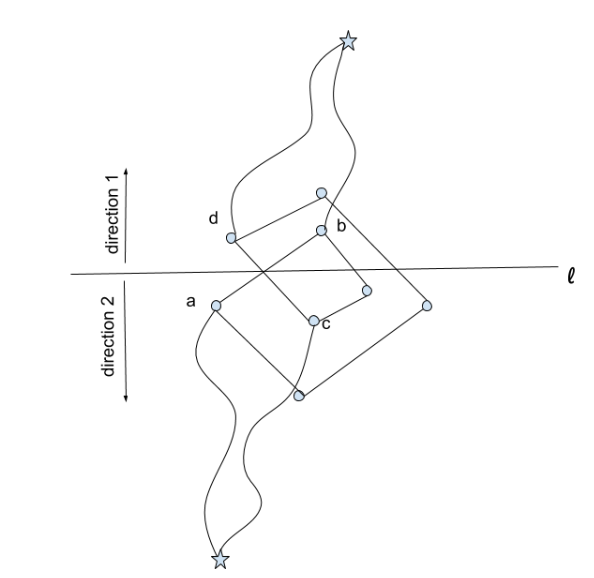
\includegraphics[scale=.7]{self_winding.PNG}
            \caption{Self winding}
    \end{figure}
    
    In the above figure, the graph G does not have any zig zag edges but has all the edges that turn in the same direction.
    
    \textbf{A winding polygon in plane is a polygon that self intersects.}
    
    Consider vertices a,b,c,d around a face and line l that separates them.
    There exist disjoint monotone paths from b to d and monotone paths from a to c. Like the previous case, we get a K4. Hence vertices a,b,c,d cannot be on a face.
    
    \begin{remark}
    If you can pick out any 4 of the vertices on a face and find two disjoint paths like shown in the below figure the 4 vertices could not have been on one face. This follows from the Jordan Curve theorem.
    \end{remark}

    \begin{figure}[H]
            \centering
            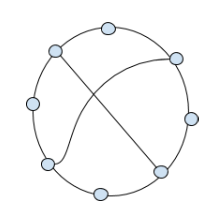
\includegraphics[scale=.8]{doublecrossingaface.PNG}
            \caption{Double crossing a face}
    \end{figure}

    In the above figure there are four vertices and two disjoint paths between them, hence it is not a face.
    
    
    \textbf{Conclusion}:
     There are no reflex vertices and there are no windings implies that the faces have to be convex.
    
    \subsection{Removing the possibility of a crossing}
    
    From the above section we know that if there are no reflex vertices and no windings(self crossings) then the faces are all convex.\\
    The next step is to show that there are not any combination of faces which when come together introduce a crossing.
    
    \begin{remark}
    Take a vertex v and consider the faces surrounding the vertex v. When you glue the faces together, the angles should sum up to ${2\pi}$.
    \end{remark}
    
    \textbf{Case I}:

    \begin{figure}[H]
            \centering
            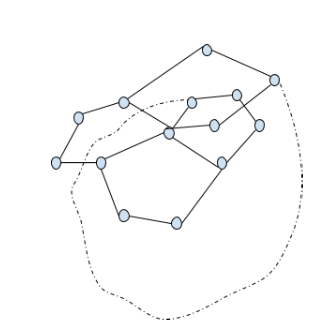
\includegraphics[scale=.8]{winding_at_a_vertex.PNG}
            \caption{Winding at a vertex}
    \end{figure}

    This is an example of another kind of winding. This would be winding in a dual.
    
    
    \textbf{Case II:}
    
    
    At any edge, both the faces that meet at an edge should be on different sides of the edge.
    
    \begin{figure}[H]
            \centering
            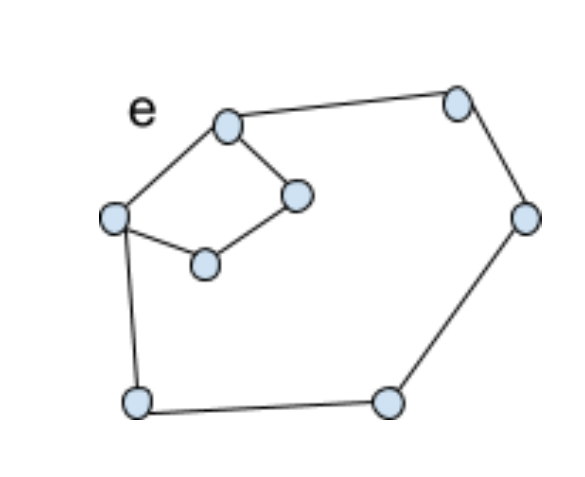
\includegraphics[scale=.5]{faces_on_same_side_of_edge.PNG}
            \caption{Faces on same side of an edge}
    \end{figure}
    
    Checking these two cases do not happen, means that everywhere locally there are no windings at any vertex and no faces such that they are on the same side of an edge.
    Globally we want to check that there are no crossings in the graph. \\
    But it will suffice to show that if these two conditions do not exist locally then globally we have faces such that they are non-overlapping.\\
    We shall discuss why these two cases cannot arise in the next lecture.

\end{document}